\textit{Results from the experiments that were considered relevant are presented here.}

\section{JNI}

\begin{figure}
    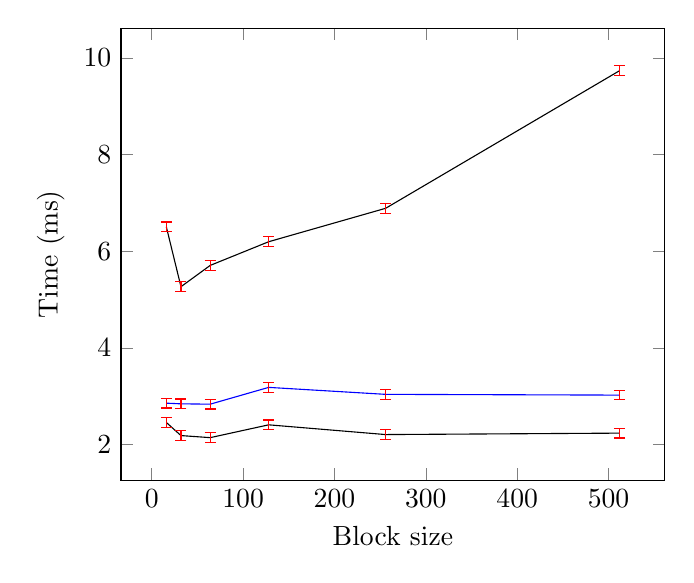
\begin{tikzpicture}
        \begin{axis}[
            xlabel={Block size},
            ylabel={Time (ms)},
            width=0.70\linewidth,
            legend pos=south east,
            scaled y ticks = false,
        ]
        \addplot [error bars/.cd, y dir=both, error bar style={red}, y explicit] coordinates {
                (16, 6.5035) +- (0.1, 0.1)
                (32, 5.2657) +- (0.1, 0.1)
                (64, 5.7065) +- (0.1, 0.1)
                (128, 6.1961) +- (0.1, 0.1)
                (256, 6.8872) +- (0.1, 0.1)
                (512, 9.7327) +- (0.1, 0.1)
                % (1024, 6.7378) +- (0.1, 0.1)
                % (2048, 5.8212) +- (0.1, 0.1)
                % (4096, 6.2328) +- (0.1, 0.1)
                % (8192, 5.6459) +- (0.1, 0.1)
                % (16384, 8.1388) +- (0.1, 0.1)
                % (32768, 10.2952) +- (0.1, 0.1)
                % (65536, 14.8090) +- (0.1, 0.1)
        };
        \addplot [error bars/.cd, y dir=both, error bar style={red}, y explicit] coordinates {
                (16, 2.4582) +- (0.1, 0.1)
                (32, 2.1875) +- (0.1, 0.1)
                (64, 2.1444) +- (0.1, 0.1)
                (128, 2.4097) +- (0.1, 0.1)
                (256, 2.2082) +- (0.1, 0.1)
                (512, 2.2379) +- (0.1, 0.1)
                % (1024, 2.2570) +- (0.1, 0.1)
                % (2048, 2.2917) +- (0.1, 0.1)
                % (4096, 2.2605) +- (0.1, 0.1)
                % (8192, 2.2291) +- (0.1, 0.1)
                % (16384, 2.2517) +- (0.1, 0.1)
                % (32768, 2.2500) +- (0.1, 0.1)
                % (65536, 2.1252) +- (0.1, 0.1)
        };
    \addplot [blue, error bars/.cd, y dir=both, error bar style={red}, y explicit] coordinates {
                (16, 2.8577) +- (0.1, 0.1)
                (32, 2.8438) +- (0.1, 0.1)
                (64, 2.8368) +- (0.1, 0.1)
                (128, 3.1840) +- (0.1, 0.1)
                (256, 3.0399) +- (0.1, 0.1)
                (512, 3.0243) +- (0.1, 0.1)
                % (1024, 4.0087) +- (0.1, 0.1)
                % (2048, 3.4426) +- (0.1, 0.1)
                % (4096, 3.4672) +- (0.1, 0.1)
                % (8192, 3.0208) +- (0.1, 0.1)
                % (16384, 5.0243) +- (0.1, 0.1)
                % (32768, 5.4063) +- (0.1, 0.1)
                % (65536, 6.4530) +- (0.1, 0.1)
        };
        % \legend{first-fit,best-fit,worst-fit,quick-fit,stdlib}
        \end{axis}
    \end{tikzpicture}
\end{figure}

\section{FFT Libraries}

\begin{figure}
    \centering
    \resizebox{\columnwidth}{!}{
        \input{Data/results/FFT/barchart_65536.tex}
    }
    \label{tab:barchart:65536}
    \caption{Bar chart for tests with block size 65536}
\end{figure}
% Which is slowest and why (discussion)??

% Which is fastest and why (discussion)??

% Which tests triggered the GC??

\section{Optimizations}
